\vspace{1cm}

\subsubsection{Login}
\begin{figure}[H]
  \centering
  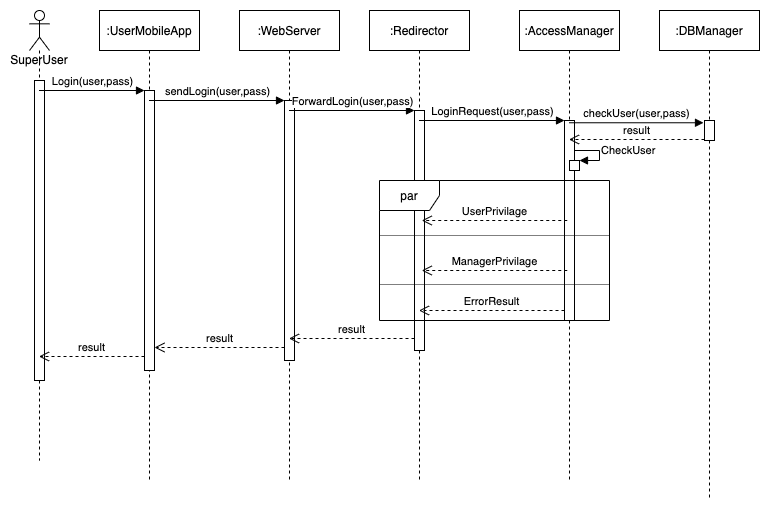
\includegraphics[width=\textwidth, keepaspectratio]{images/sequences/Login.png}
  \caption{login sequence diagram}
\end{figure}
\vspace{2cm}
In this sequence diagram is described the login process by a user.
first of all,the user login to the application through entering username and password. then it is sent to web server and after that it is forwarded to Redirector. through Redirector component, these username and passwords are sent to the right component which it is AccessManager and requested to this component by Redirector. Thus, in this step the AccessManager component checks if the user and passwords are for either users or managers or if they enter them wrong.after checking users by AccessManager, they will be sent to DBManager and forwarded to the user app, through the Redirector.

\subsubsection{GetShopList}
\begin{figure}[H]
  \centering
  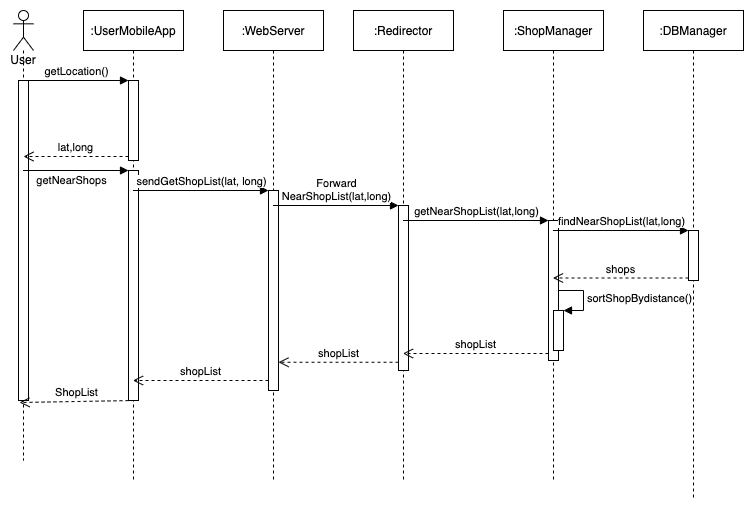
\includegraphics[width=\textwidth, keepaspectratio]{images/sequences/GetShopList.png}
  \caption{GetShopList sequence diagram}
\end{figure}
\vspace{2cm}
In this diagram, The user gets his location from the application, then through the UserMobileApp the shop lists are sent to the web server. Then the Redirector recognize that what component should do this so it will forward them to the ShopManager. As long as the shopManager gets the shop lists, through the DBManager it finds out the near shop lists and after sorting based on the distance of users, they will forwarded to the user through Redirector.

\subsubsection{AddToLineUp}
\begin{figure}[H]
  \centering
  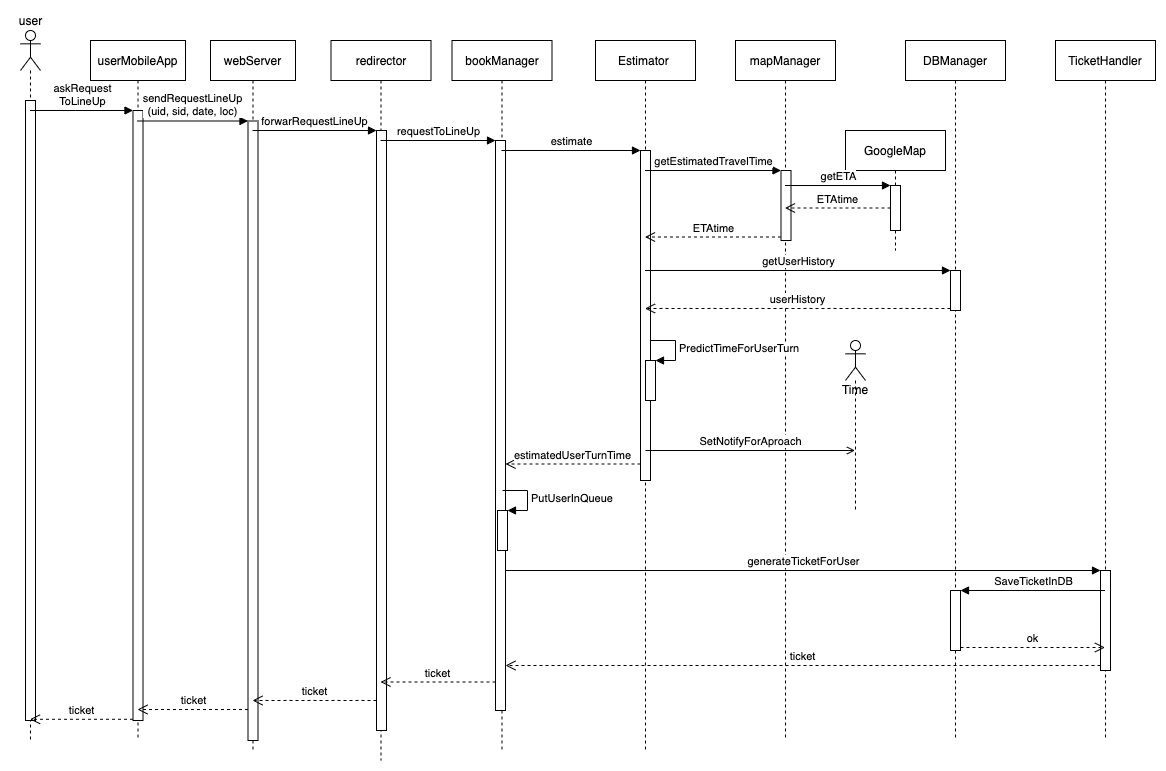
\includegraphics[width=0.9\textheight, angle=90, keepaspectratio]{images/sequences/AddToLineUp.png}
  \caption{AddToLineUp sequence diagram}
\end{figure}
\vspace{2cm}
In this diagram,firstly the user asks to request for lining up, then like the previous diagram,it sends the request to web server and through Redirector, it is chosen to send the request to bookManager. Then, Estimator component get estimated time of arrival from the mapManger to manage the location of the user and within using that it can estimate the proper time. Meanwhile the mapManager use google map for this part. Also the Estimator set a notification to send it to the users. After all the bookManager generate a ticket for users by TicketHandler and thus forward to the user.\\ \\

For the two next diagram its almost the same, just the concept is a little bit different, which for the second one is booking a visit with the same procedure and the third one is exactly like the first one except the process id offline in the third one.

\subsubsection{BookAVisit}
\begin{figure}[H]
  \centering
  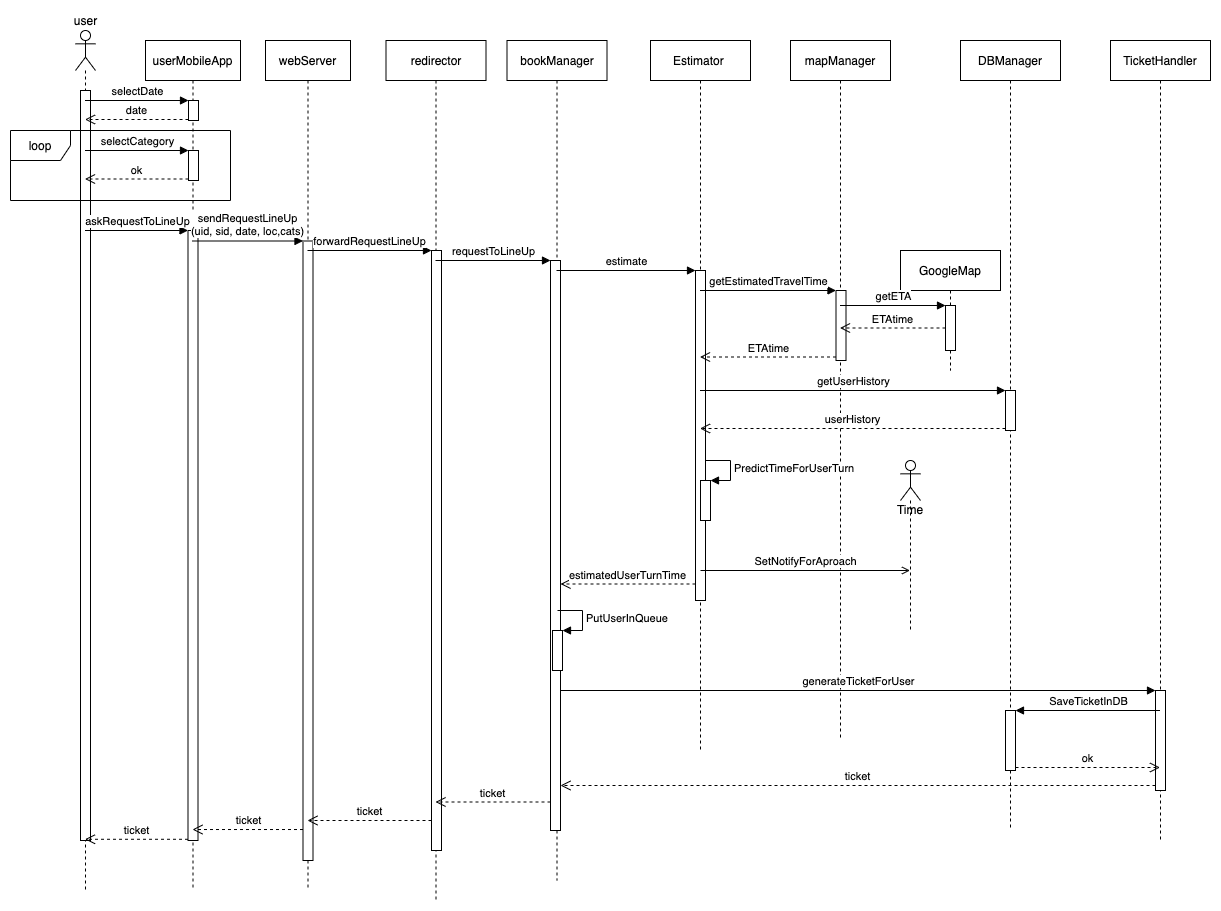
\includegraphics[width=0.9\textheight, angle=90, keepaspectratio]{images/sequences/BookAVisit.png}
  \caption{BookAVisit sequence diagram}
\end{figure}
\vspace{2cm}

\subsubsection{OfflineLineUp}
\begin{figure}[H]
  \centering
  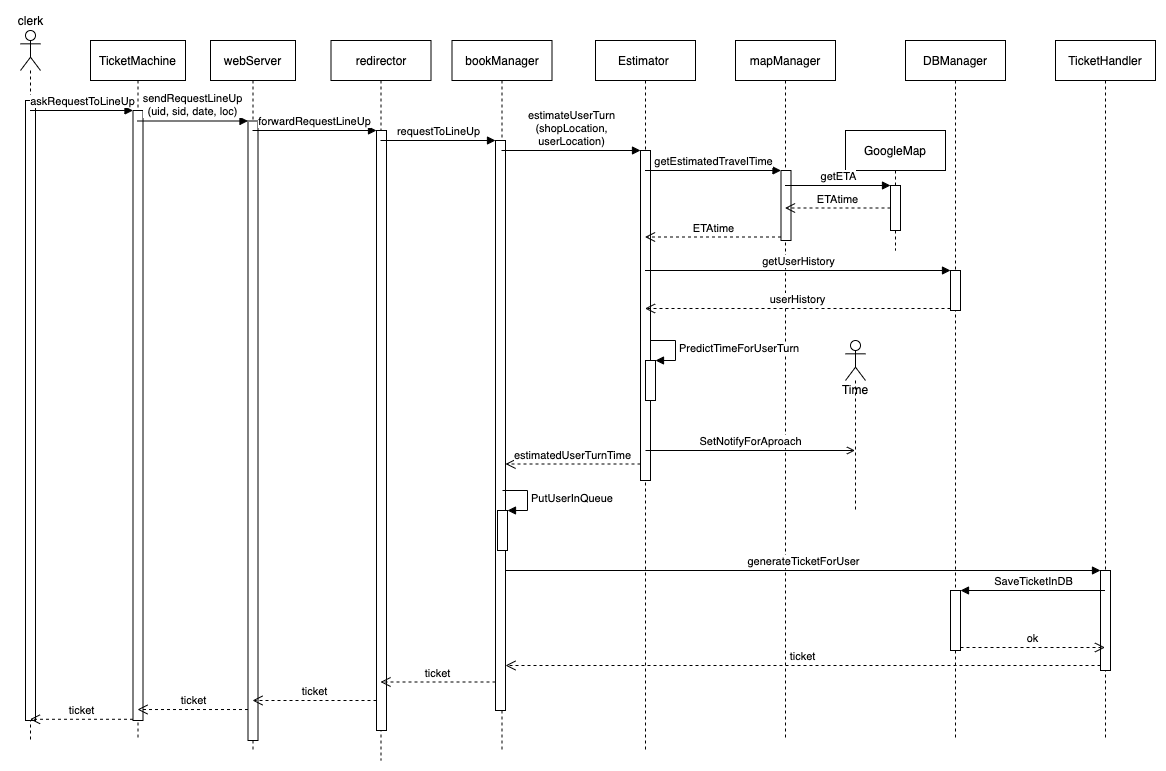
\includegraphics[width=0.9\textheight, angle=90, keepaspectratio]{images/sequences/OfflineLineUp.png}
  \caption{OfflineLineUp sequence diagram}
\end{figure}
\vspace{2cm}

\subsubsection{Enter}
\begin{figure}[H]
  \centering
  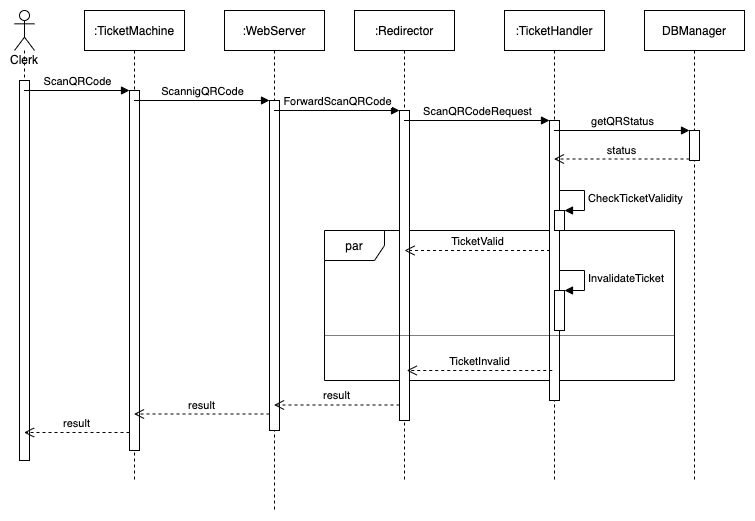
\includegraphics[width=\textwidth, keepaspectratio]{images/sequences/Enter.png}
  \caption{Enter sequence diagram}
\end{figure}
\vspace{2cm}
In this diagram, the clerk scan the QR codes through ticketMachine. It then goes through web server and through director it is forwarded to tickrtHandler and will check if its valid or not. Thus after getting by DBManager, the result is going to be forwarded to clerk.


\subsubsection{Checkout}
\begin{figure}[H]
  \centering
  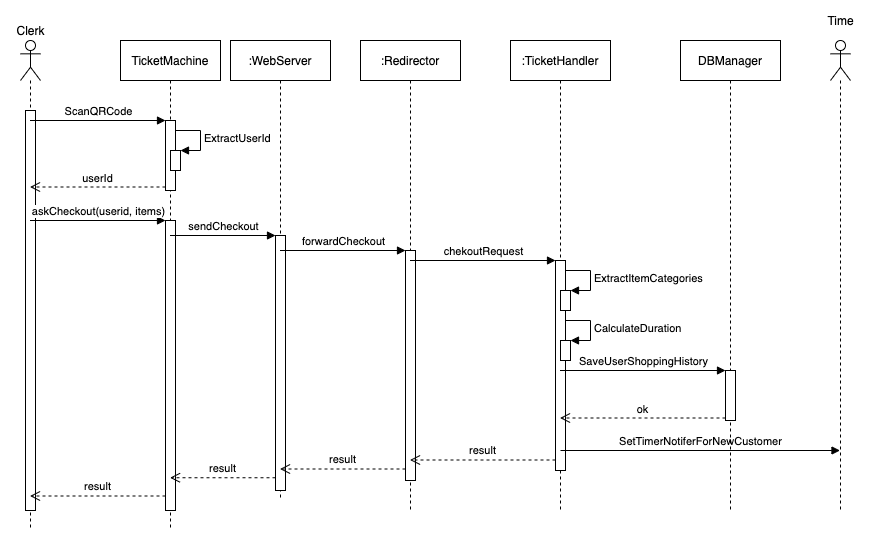
\includegraphics[width=\textwidth, keepaspectratio]{images/sequences/Checkout.png}
  \caption{Checkout sequence diagram}
\end{figure}
\vspace{2cm}
For checking out diagram, its almost like the previous one, except some differences. One of them is that the ticketHandler recognize the duration of shopping and will calculate it and also extract the item categories chosen by users.Moreover the ticketMachine also extract users id at the beginning.

\clearpage

\subsection{Component Interfaces}
In the next diagram are described the main methods which can be invoked on the interfaces and their interactions, referring to the most important processes reported in the runtime view section.
\vspace{2cm}
\begin{figure}[H]
  \centering
  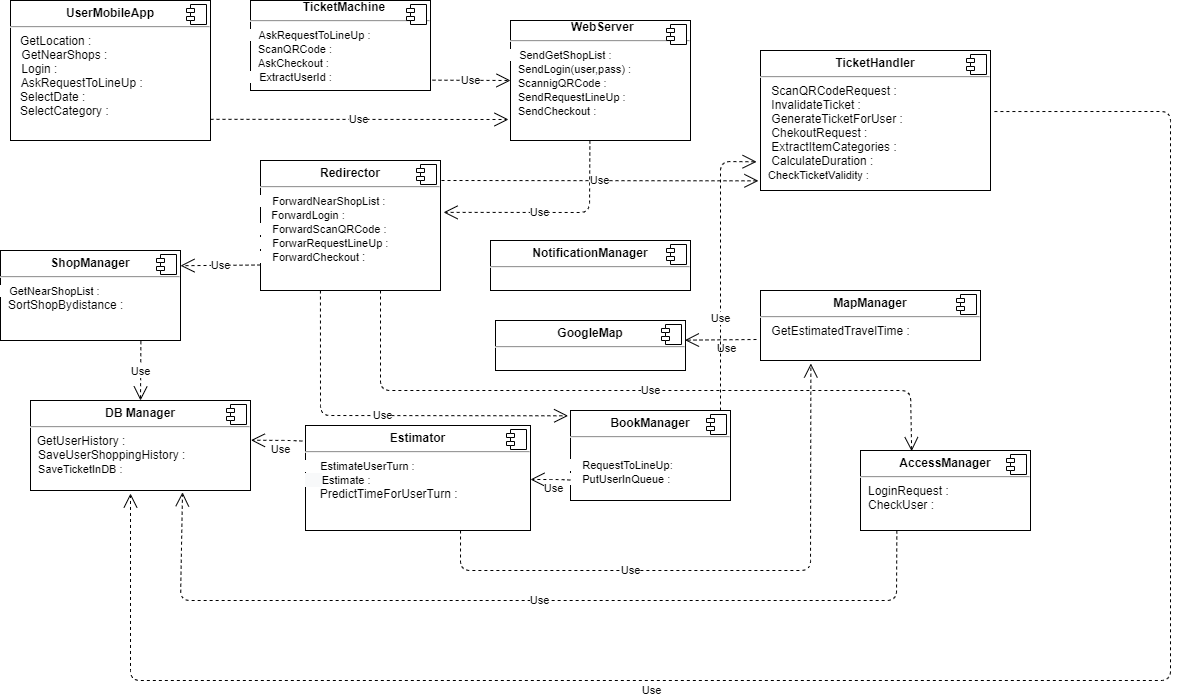
\includegraphics[width=1.1\textwidth, keepaspectratio]{images/Component Interfaces.png}
  \caption{Component Interface Diagram}
\end{figure}
\vspace{2cm}